\section{Details on user studies for the agent interface}
\label{user_study}
Below we describe the exact guideline definitions we shared with the user for a user study.

\subsubsection{Hypothesized Frustrations}
We presented participants with the following hypothesized frustrations related to T2I model usage:
\begin{enumerate}
\item \textbf{Prompt Misinterpretation:} The model misunderstands complex relationships between entities in the input prompt.
\item \textbf{Many Prompt Iterations:} The model does not immediately generate what the user intends, requiring numerous iterative changes to the input prompt.
\item \textbf{Inconsistent Generations:} The model reinterprets the input prompt differently between iterations, causing unwanted changes in the generated images.
\item \textbf{Incorrect Assumptions:} The model makes incorrect assumptions or no assumptions when encountering gaps in the details provided in the input prompt, leading to undesired outputs.
\end{enumerate}

Explanations of terms were given to users of: 
\begin{enumerate}
\item "Entities" are single items that are intended to be in the image e.g. "Cat" and "Ball", from "make a sketch of a Cat playing with a Ball"
\item "Prompt" means the text written to communicate the intended output image e.g. the sentence "make a sketch of a Cat playing with a Ball" is the "Prompt", also known as "Input" 
\item "Iterations" are each set of different image outputs by the model, taken from a different input, or even the same input just regenerated
\end{enumerate}

The question asked for each Frustration were: "Please score the below frustrations (or issues) that could be related to Text to Image AI Generation"."Rank in terms of how much they relate to your current usage, with your most commonly used model or app." 




\subsubsection{Hypothesized Features}
We proposed the following features as potential solutions to address the identified frustrations:
\begin{enumerate}
\item \textbf{Clarifications:} The model would ask specific clarifying questions about uncertainties in the prompt.  These details would then be incorporated into subsequent iterations. For example: "Is the cat playing with: 1. a ball of wool, or 2. a tennis ball?"
\item \textbf{Graph of Prompt Entities:}  A visual representation of all entities in the prompt as a graph, allowing users to see and edit attributes of each entity.  E.g., seeing that the model has assigned "round," "small," and "wooden" as attributes to "table" and allowing the user to change them to "square" and "metal."
\item \textbf{Graph of Prompt Relationships:} A visual representation of relationships between entities in the prompt, allowing users to see and edit these relationships. E.g., seeing that "donut" is "next to" "coffee" and allowing the user to change the relationship to "on top of."
\end{enumerate}

The questions asked for each feature were: 
\begin{enumerate}
\item "How likely this feature is to help your current workflow if you had it now?". With response options of: "Very unlikely to help", "Unlikely to help", "Could help", "Likely to help", "Very likely to help". 
\item "How soon would this feature deliver value to your work?" with response options of: "Very soon / immediately", "Sometime, "Not very soon".
\end{enumerate}

Image references were given for each Feature as listed out below:

\begin{enumerate}
\item \textbf{Clarifications:} 
\begin{figure} [H]
    \centering
    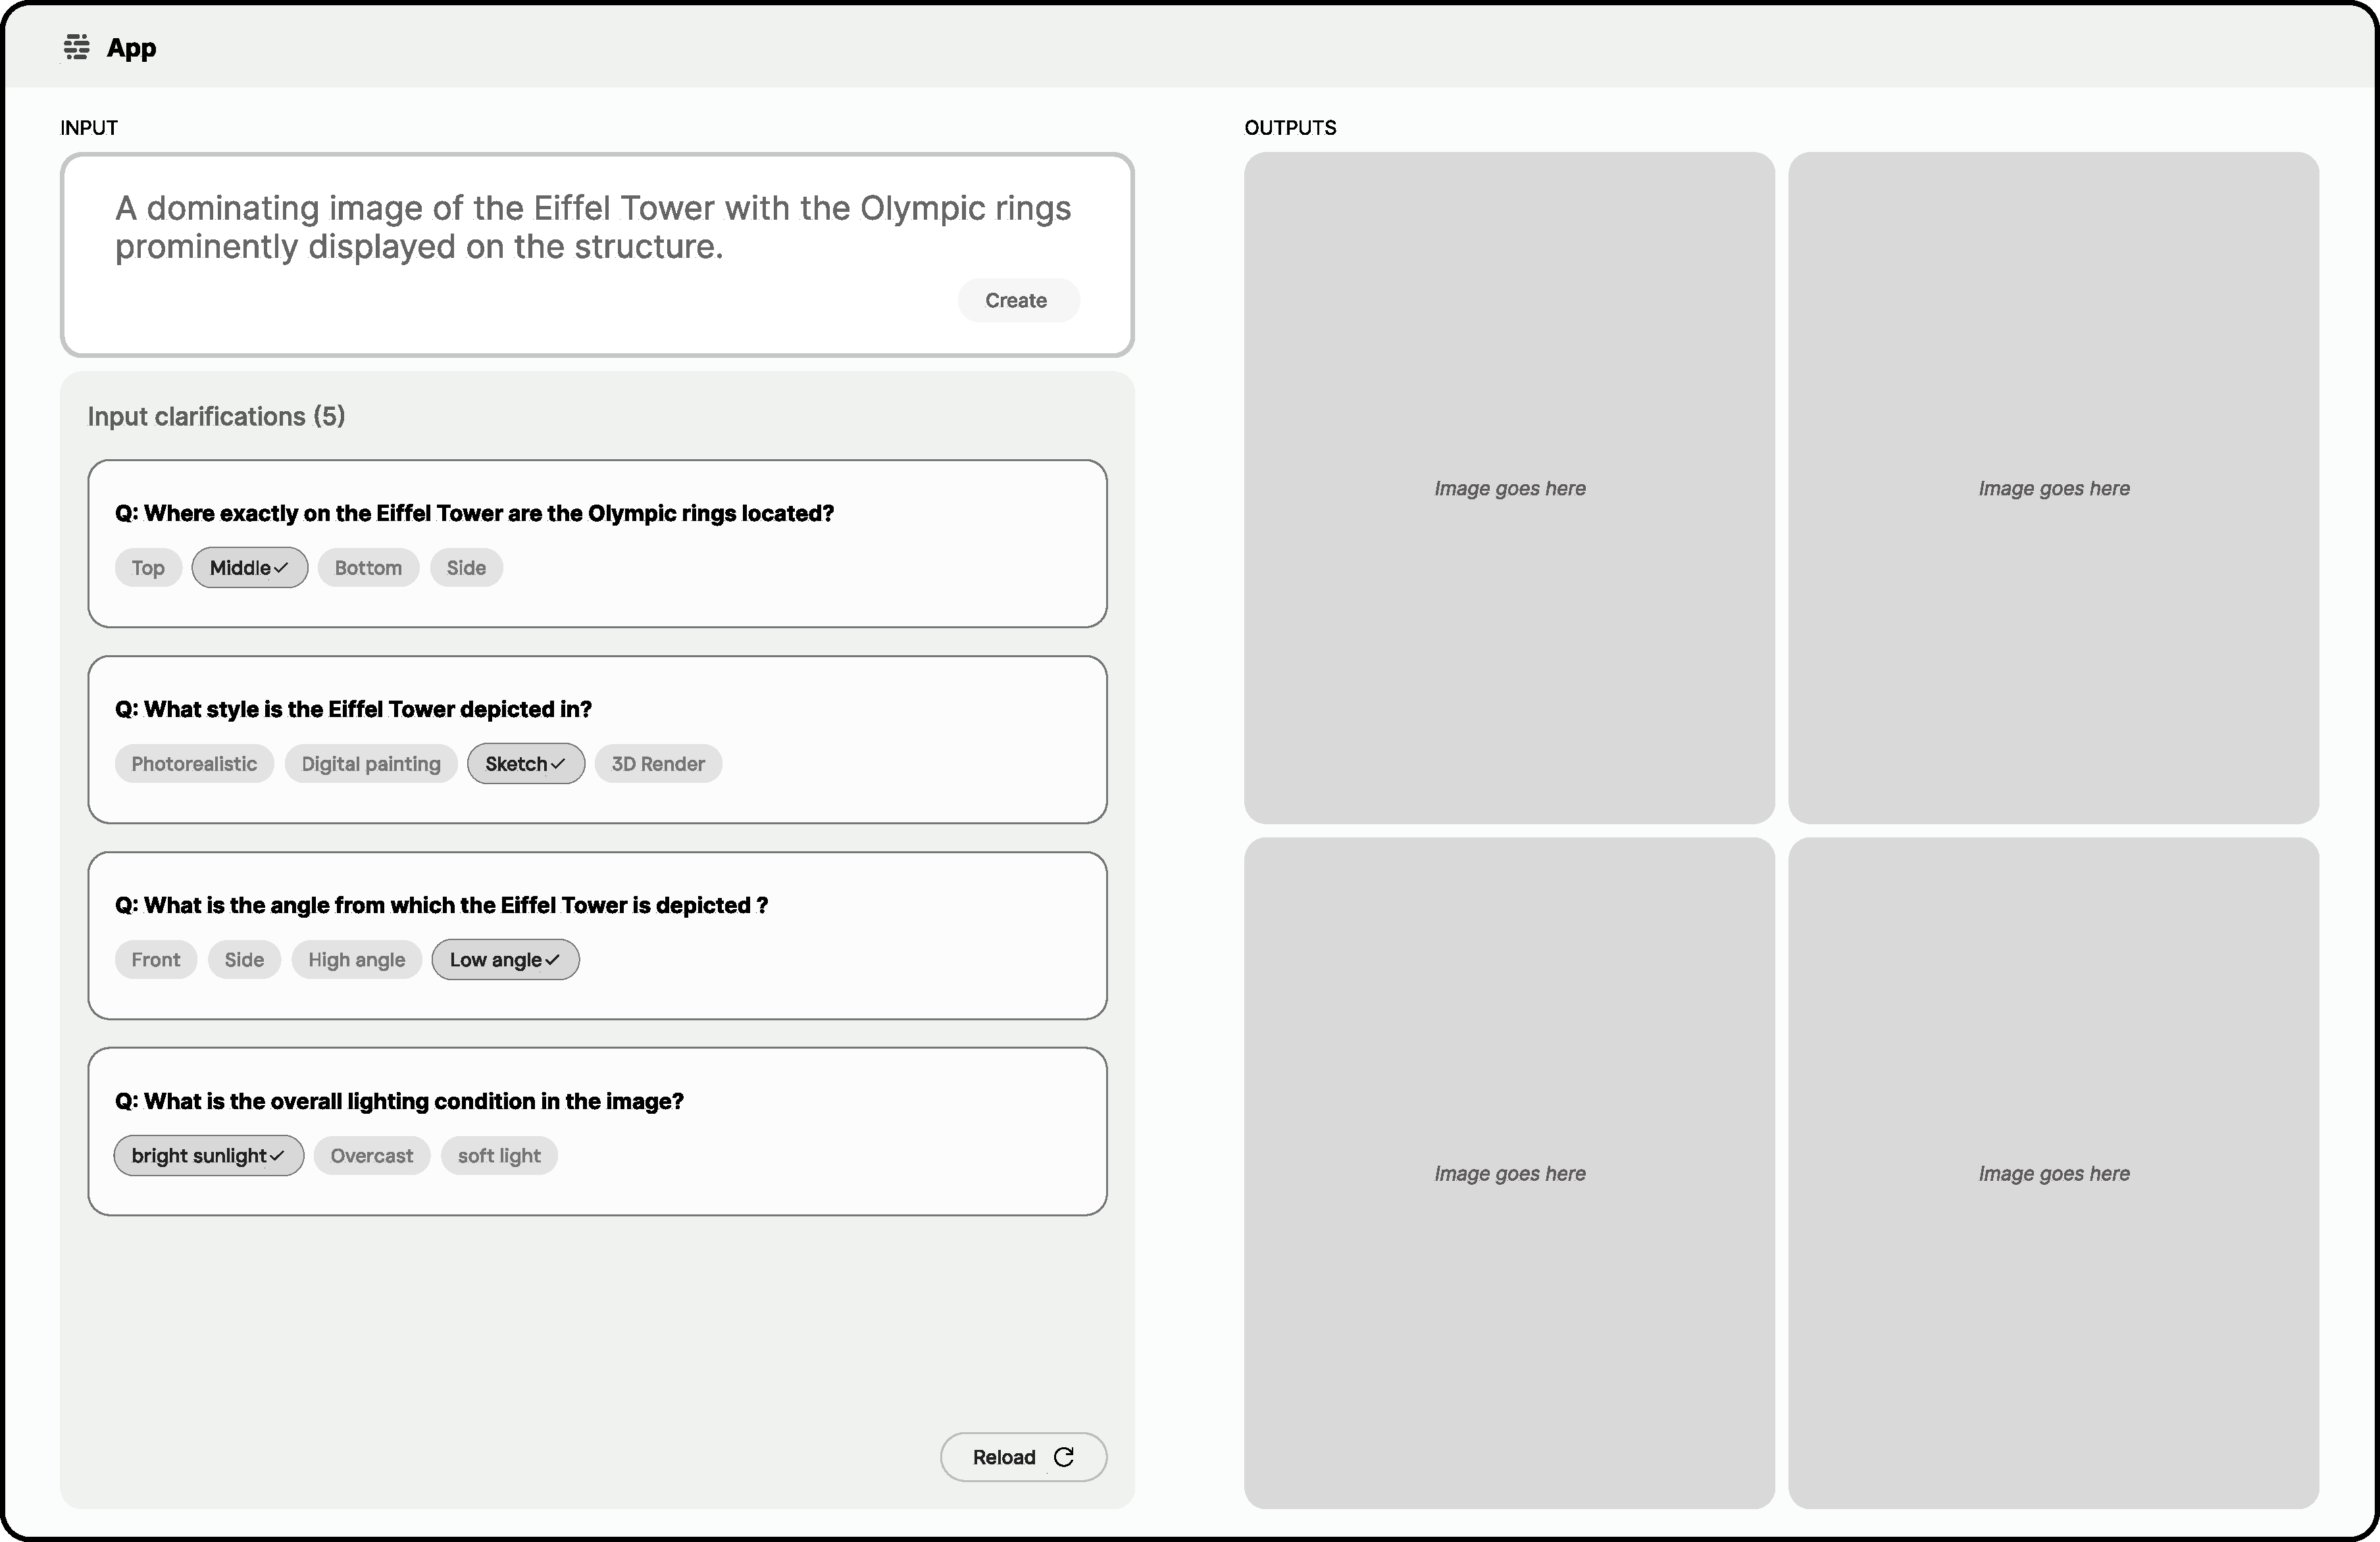
\includegraphics[width=.9\linewidth]{figures/F1_Questions.pdf}
    \caption{Stimulus image in the survey to test the Model clarifications feature.}
    \label{fig:interface-human}
\end{figure} 

\clearpage
\item \textbf{Graph of Prompt Entities:}  
\begin{figure} [H]
    \centering
    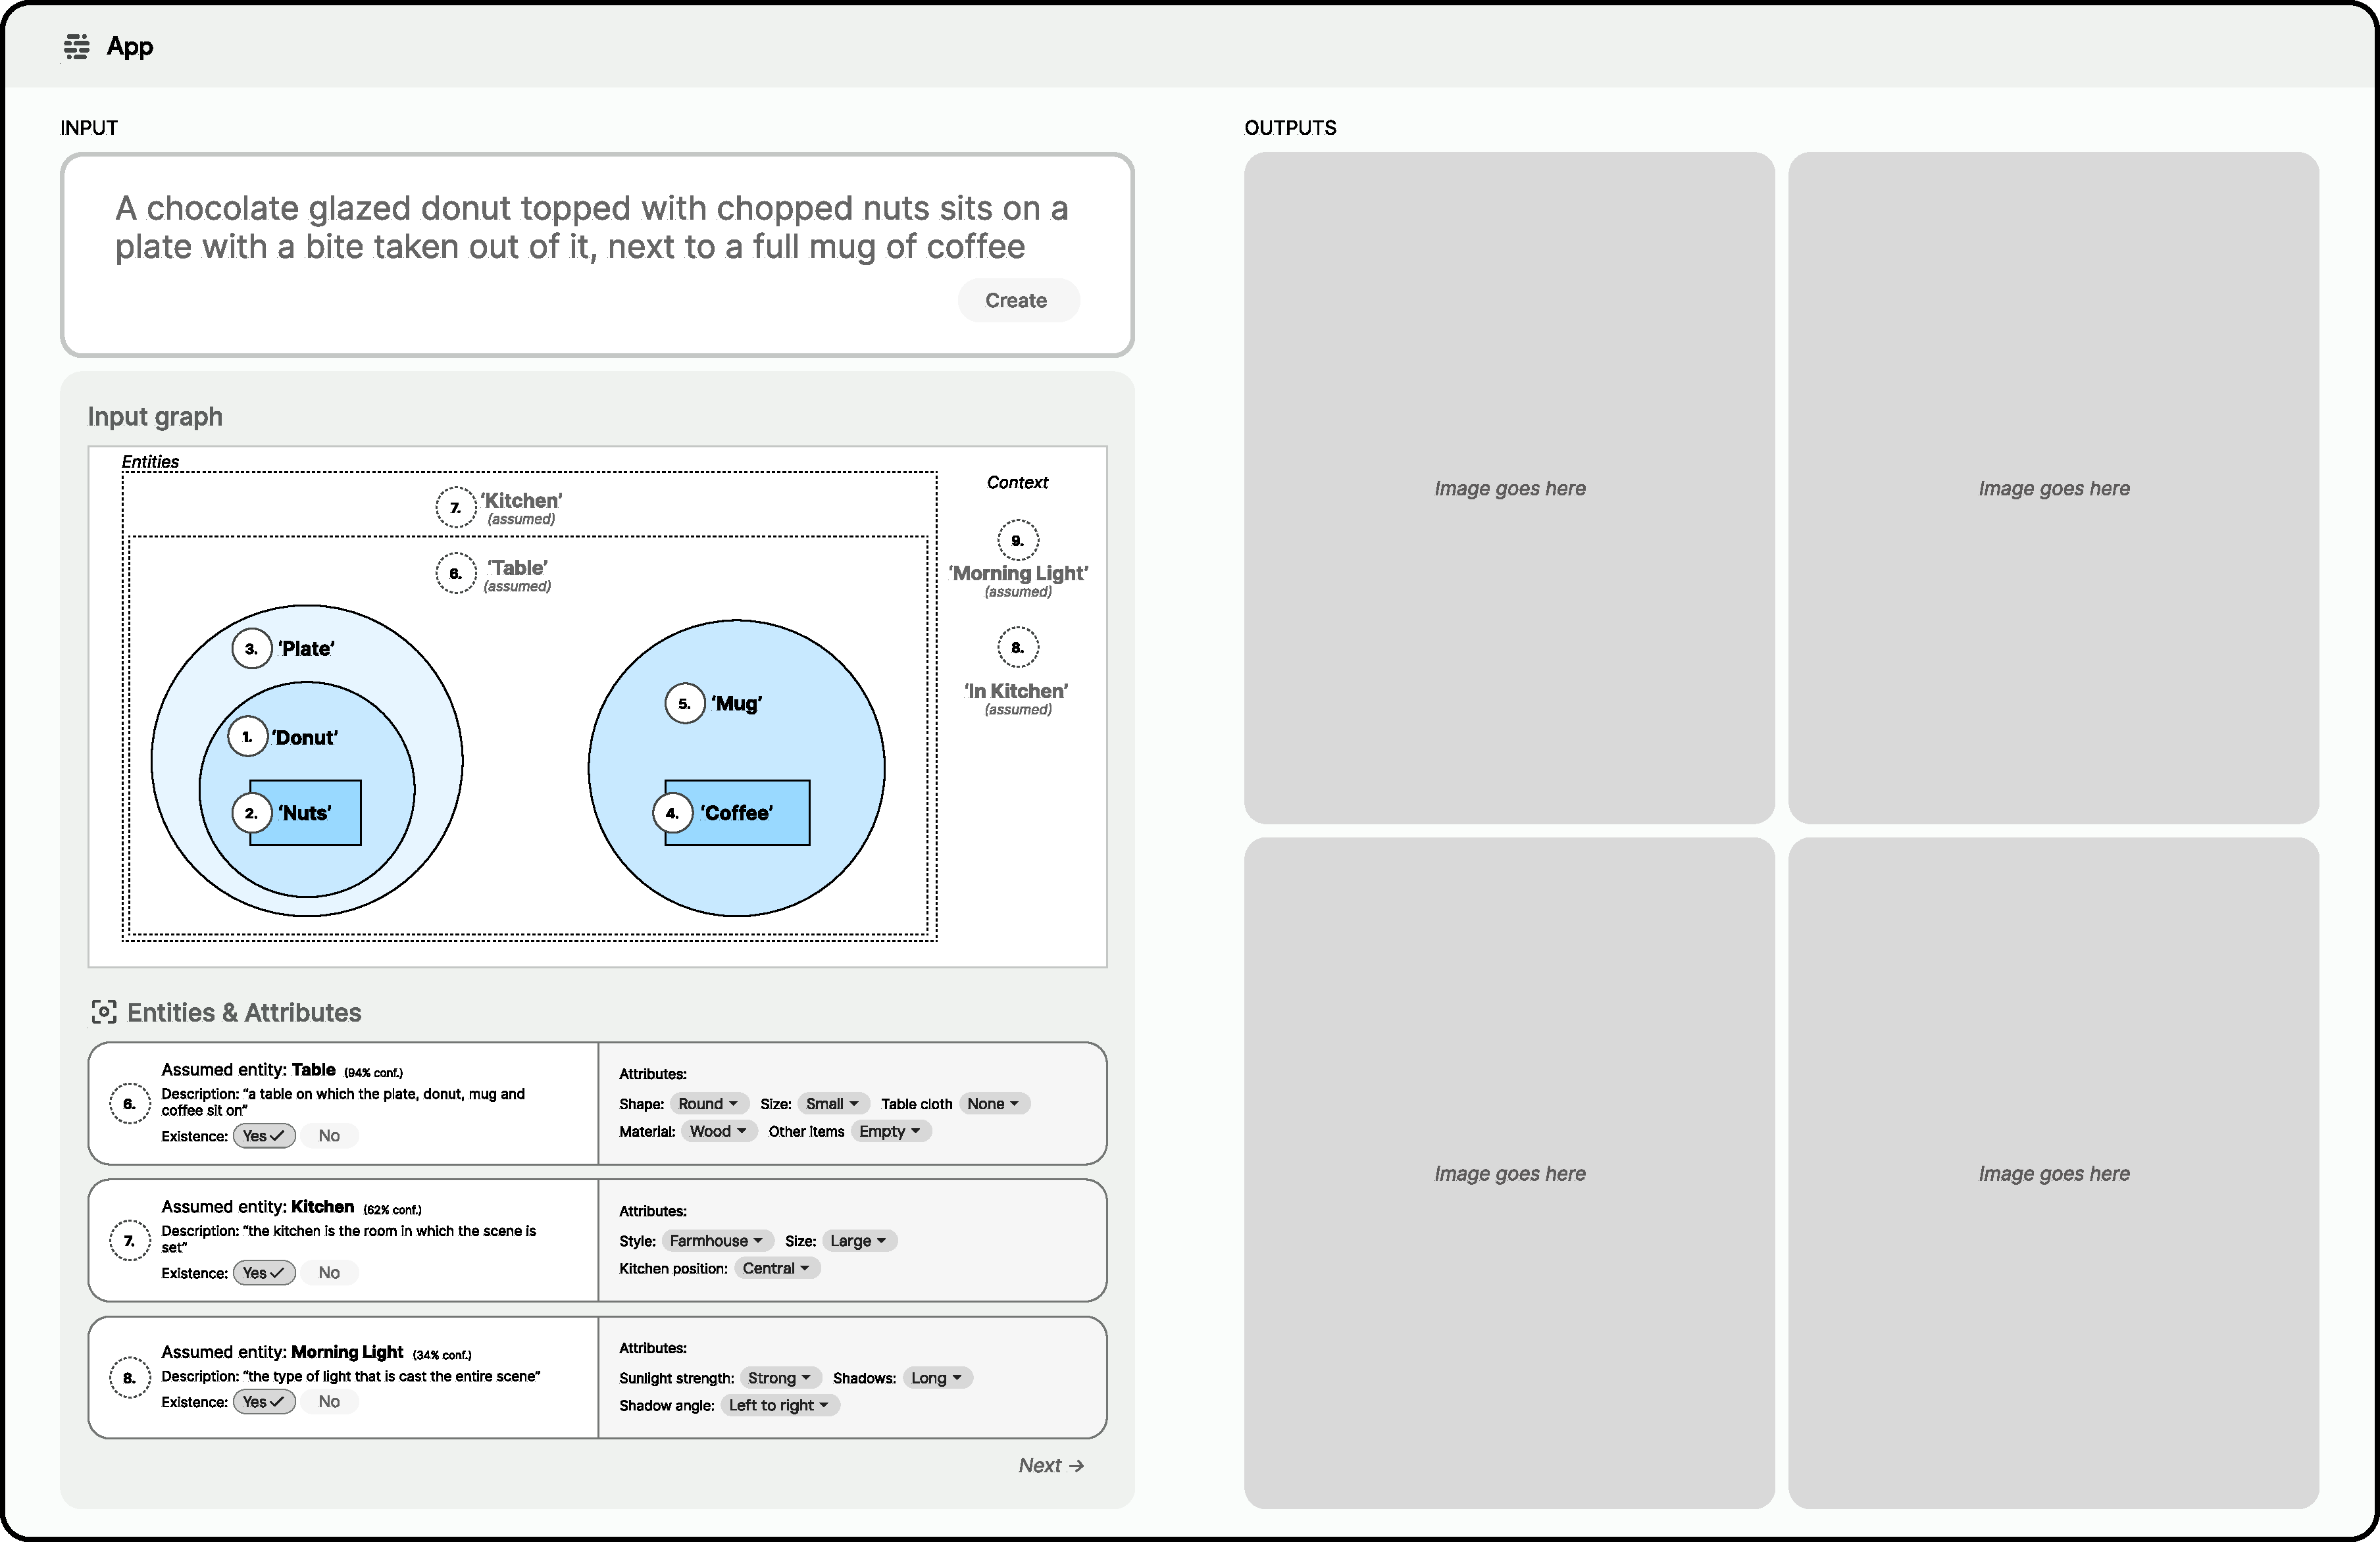
\includegraphics[width=.9\linewidth]{figures/F2_Graph.pdf}
    \caption{Stimulus image in the survey to test the Model Graph of Entities and Attributes feature.}
    \label{fig:interface-human2}
\end{figure} 

\item \textbf{Graph of Prompt Relationships:} 
\begin{figure} [H]
    \centering
    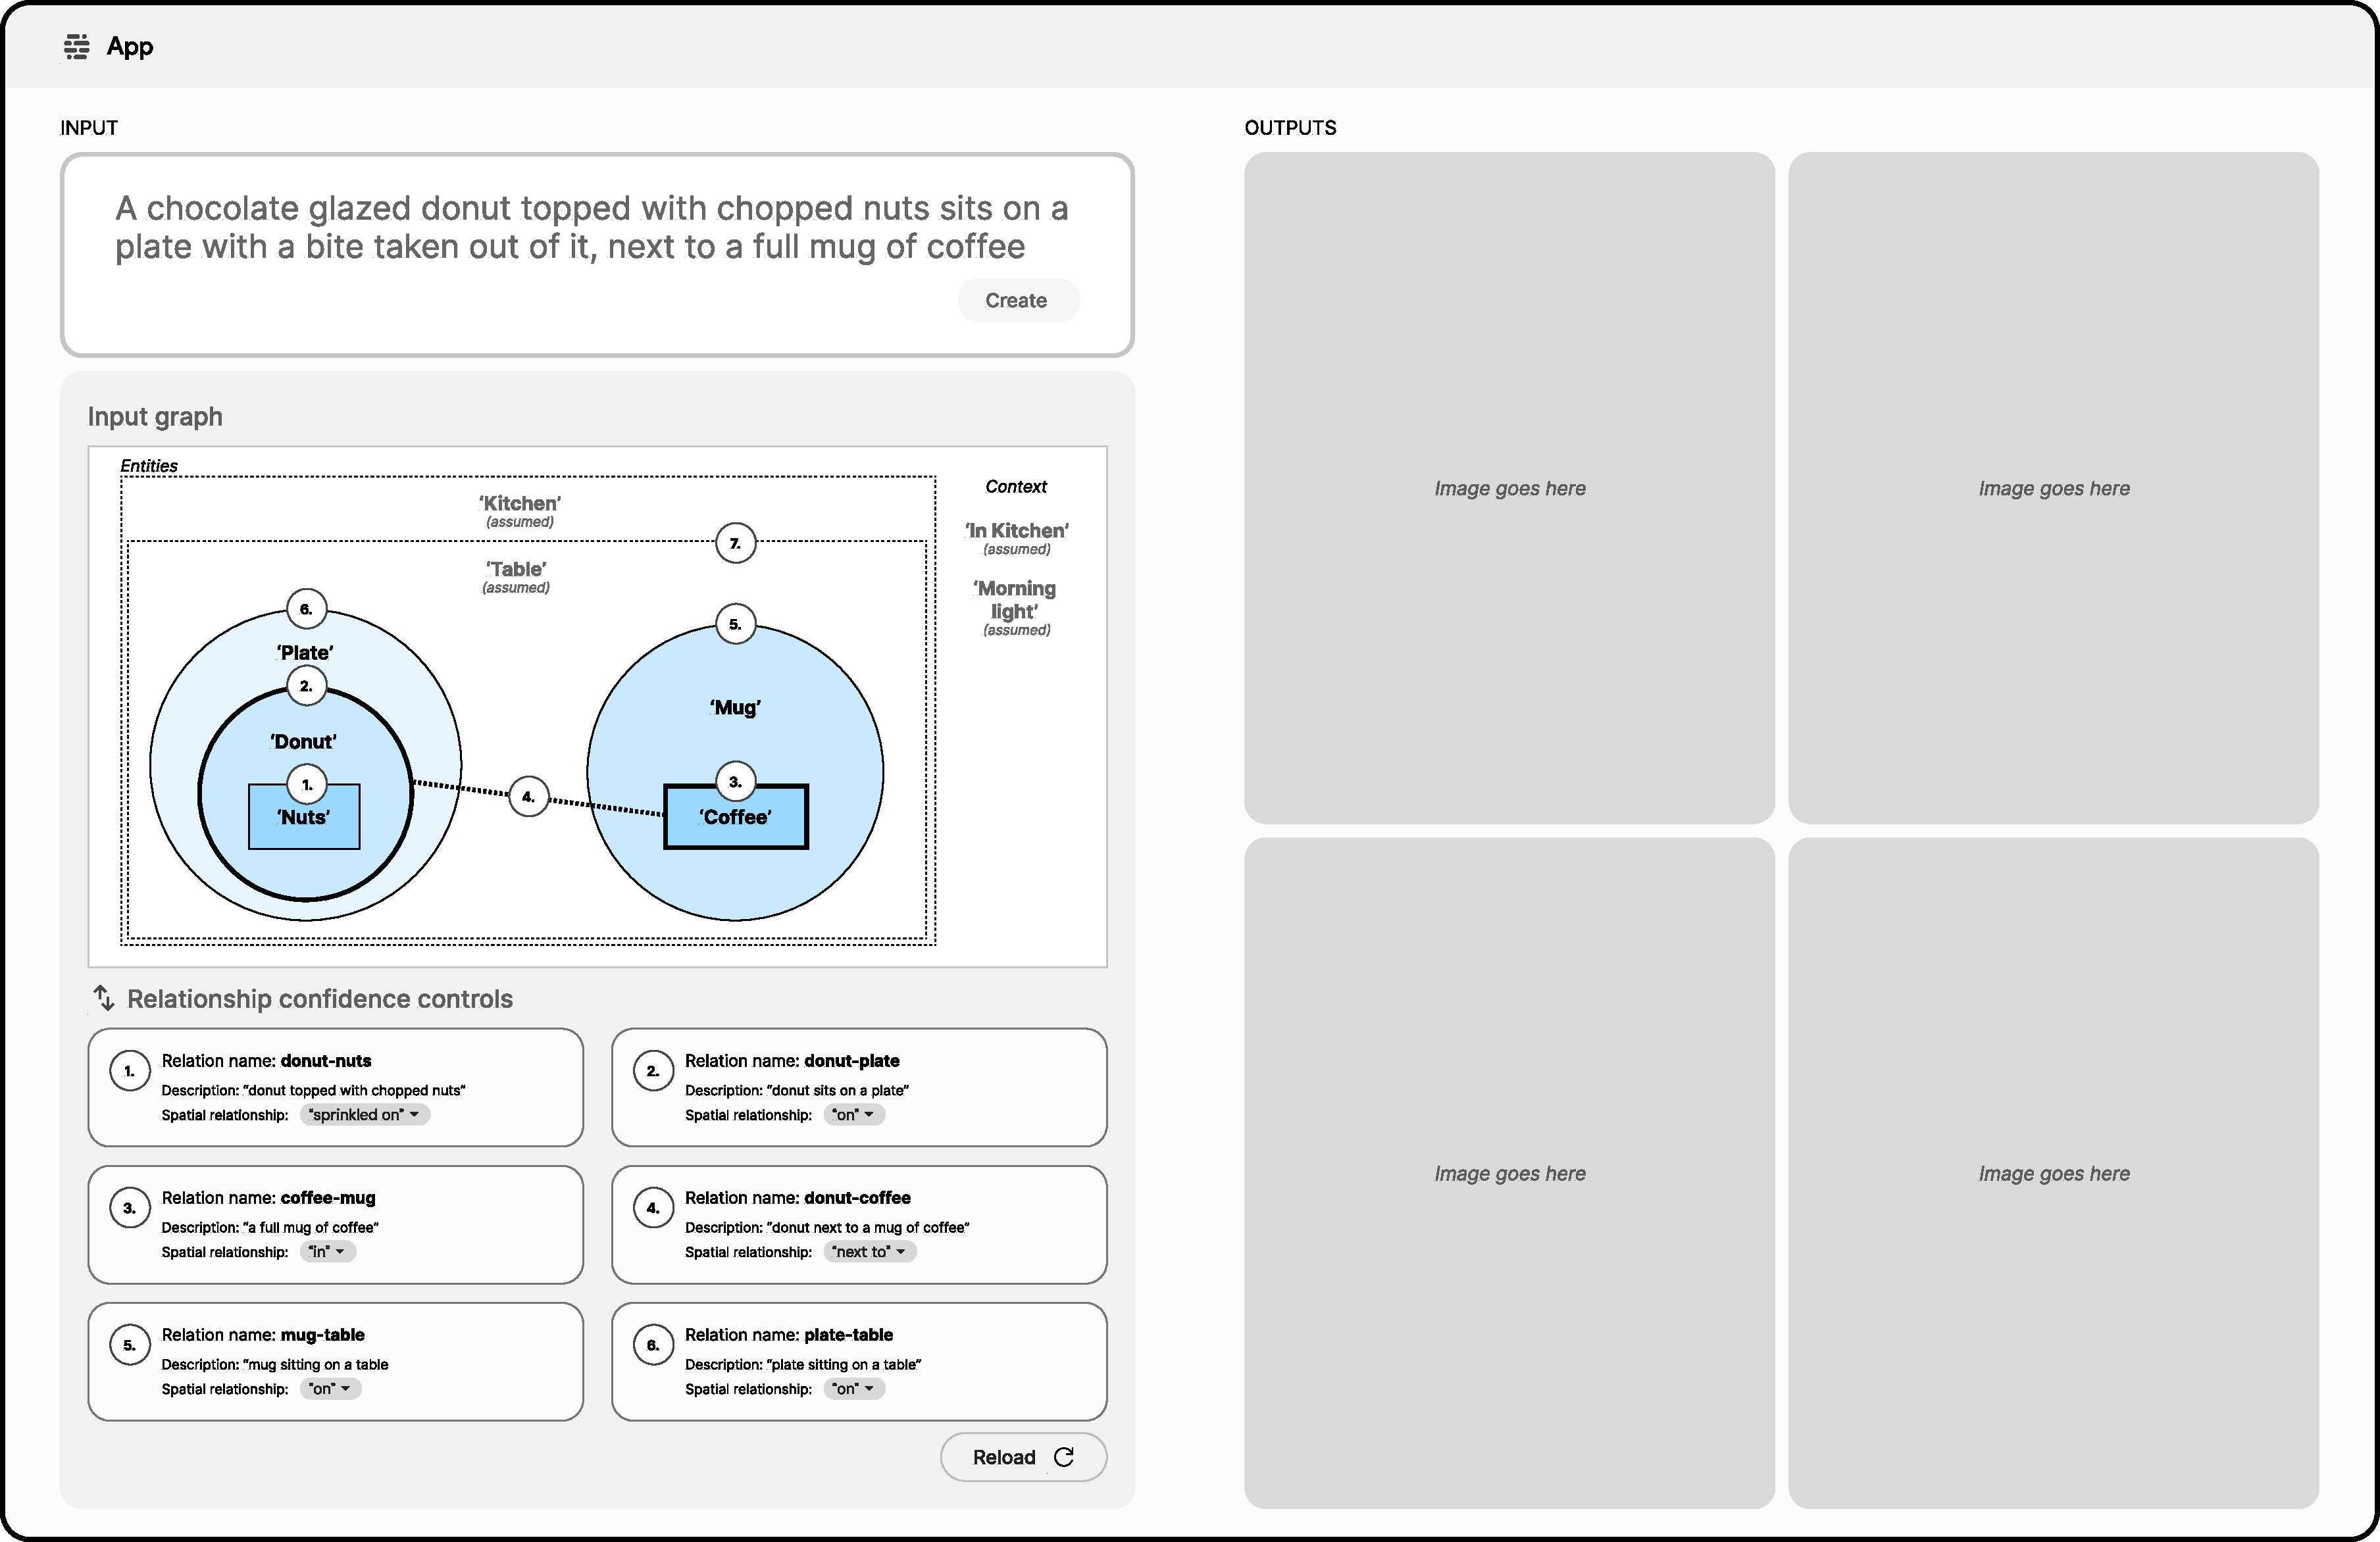
\includegraphics[width=.9\linewidth]{figures/F3_Relations.pdf}
    \caption{Stimulus image in the survey to test the Model Graph of Entity Relations feature.}
    \label{fig:interface-human3}
\end{figure} 

\end{enumerate}

\subsubsection{Human Study Results}
\Cref{tab:t2i_frequency} details the T2I usage frequency of the human subjects. \Cref{table_frustration1} shows the percentage of human subjects that reported different kinds of frustrations in their experience of using T2I. \Cref{table_frustration2} summarizes the results on expected speed of value delivered from different features of our agent prototypes. These results highlight the impact of our contributions.
\begin{table}[h]
\caption{Breakdown of the T2I usage frequency of the 143 participants recorded}
\centering
\label{tab:t2i_frequency}
\begin{tabular}{lrr} 
\toprule
\textbf{Usage Frequency} & \textbf{No. of participants} & \textbf{(\%)} \\
\midrule
Many times a day & 13 & 9.1 \\ 
Many times a week & 44 & 30.8 \\
At least once a week & 36 & 25.2 \\
At least once a month & 50 & 35.0 \\
\bottomrule
\end{tabular}
\end{table}


\begin{table}[h]
\caption{Reported User Frustrations with existing T2I processes (\% of participants)}
\centering
\small
\begin{tabular}{lccccc} %
\toprule
\textbf{Frustration} & \textbf{V. Freq. (\%)} & \textbf{Freq. (\%)} & \textbf{Occas. (\%)} & \textbf{V. Occas. (\%)} & \textbf{No Issue (\%)} \\ %
\midrule
Prompt Misinterpret. & 7 & 19.6 & 43.4 & 23.1 & 7 \\  %
Many Iterations & 10.5 & 44.8 & 28 & 11.9 & 4.9 \\ %
Inconsistent Gen. & 11.2 & 20.3 & 39.9 & 21 & 7.7 \\ %
Incorrect Assumptions & 7 & 23.1 & 39.2 & 20.3 & 10.5 \\ %
\bottomrule
\end{tabular}
\label{table_frustration1}  %
\end{table}


\begin{table}[h]
\caption{Expected speed of value delivered from features (\% of users)}
\centering
\small
\begin{tabular}{lccccc} %
\toprule
\textbf{Feature} & \textbf{Very soon / immediately (\%)} & \textbf{Sometime(\%)} & \textbf{Not very soon. (\%)}
\\ %
\midrule
Clarifications & 57.7 & 37.2 & 5.1 \\  %
Entity Graph & 49.6 & 34.8 & 15.6 \\ %
Relation Graph & 41.8 & 44 & 14.2 \\ %
\bottomrule
\end{tabular}
\label{table_frustration2}  %
\end{table}


\clearpage
\textbf{Template of Human Rater Task 1: Evaluation of Issues in Individual Questions} 
\begin{figure} [H]
    \centering
    \includegraphics[width=.9\linewidth]{figures/Task_1.pdf}
    \caption{An example of the template presented to human raters. Human raters are asked to mark any issues a question contains that could pose a disturbance to the user. Approximately 8k questions per Agent are rated. The results are shown in \Cref{fig:rating_human_dialog}.}
    \label{fig:interface-human-model-task-1}
\end{figure} 
\clearpage

\textbf{Template of Human Rater Task 2: Evaluation of Similarity between the generated image and the Human-AI dialog and the original prompt.} 
\begin{figure} [H]
    \centering
    \includegraphics[width=.9\linewidth]{figures/Task_2.pdf}
    \caption{An example of the template presented to human raters. Human raters are asked to rank the correspondence of each image to the agent-user dialog and original prompt. Approximately 1.5k image-dialog pairs are rated using 3 human raters. Results in \Cref{fig:rating_human_dialog}.}
    \label{fig:interface-human-model-task-2}
\end{figure} 
\clearpage


\textbf{Template of Human Rater Task 3: Evaluation of the generated image similarity to the goal image.} 
\begin{figure} [H]
    \centering
    \includegraphics[width=.9\linewidth]{figures/Task_3.pdf}
    \caption{A template of the task presented to human raters. Human raters are asked to rate the images produced by the three proposed multi-turn agents and a single-turn T2I model against a Ground Truth image for which the original prompt was derived and the answers to the agents questions were derived. Approximately 550 image-dialog pairs per agent are rated using 3 human raters. The generated images were presented in a random order and were unlabeled and the human rater was tasked with ranking the images from best to worst. The results from the study are shown in \Cref{fig:rating_human_rank}.}
    \label{fig:interface-human-model-task-3}
\end{figure} 
